\documentclass[10pt,a4paper]{article}
\usepackage[margin=1.9cm]{geometry}
\usepackage[T1]{fontenc}
\usepackage{lmodern}
\usepackage{amsmath}
\usepackage{xcolor}
\usepackage{tikz}
\usetikzlibrary{shapes.geometric, arrows.meta, positioning, calc}
\usepackage{booktabs}
\usepackage{array}
\usepackage{enumitem}
\usepackage{titlesec}

\definecolor{fpgablue}{RGB}{13,71,161}
\definecolor{fpgalight}{RGB}{187,222,251}
\definecolor{hostgreen}{RGB}{27,94,32}
\definecolor{hostlight}{RGB}{200,230,201}
\definecolor{accent}{RGB}{183,28,28}
\definecolor{rulegray}{RGB}{120,120,120}
\definecolor{noteyellow}{RGB}{255,249,196}
\definecolor{noteborder}{RGB}{255,193,7}

\usepackage[colorlinks=true]{hyperref}
\hypersetup{linkcolor=fpgablue, urlcolor=blue,
            pdftitle={FPGA Tick-to-Trade Technical Brief}}

\setlength{\parindent}{0pt}
\setlength{\parskip}{5pt}

\titleformat{\section}{\large\bfseries\color{fpgablue}}{\thesection.}{0.5em}{}
\titleformat{\subsection}{\normalsize\bfseries\color{fpgablue}}{}{0em}{}
\titlespacing*{\section}{0pt}{10pt}{4pt}
\titlespacing*{\subsection}{0pt}{6pt}{2pt}

\tikzset{
  blk/.style={rectangle, rounded corners=3pt, draw=fpgablue, fill=fpgalight,
    text=fpgablue, font=\scriptsize\bfseries, align=center,
    minimum height=0.95cm, minimum width=2.05cm},
  hostblk/.style={rectangle, rounded corners=3pt, draw=hostgreen, fill=hostlight,
    text=hostgreen, font=\scriptsize\bfseries, align=center,
    minimum height=0.95cm, minimum width=2.05cm},
  io/.style={rectangle, draw=rulegray, fill=gray!8, font=\scriptsize, align=center,
    minimum height=0.95cm, minimum width=1.7cm},
  note/.style={rectangle, rounded corners=2pt, draw=noteborder, fill=noteyellow,
    font=\scriptsize, align=left, inner sep=5pt},
  fa/.style={-{Stealth[length=5pt]}, line width=1pt, color=fpgablue},
  ga/.style={-{Stealth[length=5pt]}, line width=1pt, color=hostgreen},
}

\newcommand{\hruleline}{\textcolor{rulegray}{\rule{\linewidth}{1pt}}}

\begin{document}

% ============================ HEADER =======================================
{\LARGE\bfseries\color{fpgablue} FPGA Tick-to-Trade}\hfill
{\small\color{rulegray} Technical Brief \textbullet\ June 2026}\\[-1pt]
{\large A hardware trading pipeline: NASDAQ ITCH in, order decision out, in \textbf{195\,ns}.}

\hruleline

\vspace{-2pt}
This system reconstructs the NASDAQ order book and emits a trading decision
\textbf{entirely in FPGA fabric}, on a fixed, jitter-free 195\,ns budget --- roughly
\textbf{five orders of magnitude} faster than the equivalent software path. It targets
AWS F1 (Xilinx UltraScale+ VU9P), is verified bit-for-bit against a Python golden model,
and routes its decisions to a live Interactive Brokers \emph{paper} account. This brief
is the map; the three detailed parts (architecture, RTL \& verification, integration)
are the territory.

% ============================ ARCHITECTURE ==================================
\section{System architecture}

The design has two paths. The \textbf{hardware fast path} (blue) turns a raw market-data
byte stream into a trade decision in 195\,ns. The \textbf{software execution path} (green)
takes that decision off-chip and routes it to the broker --- network-bound at tens of
milliseconds. The whole point of the project lives in the gap between the two.

\begin{center}
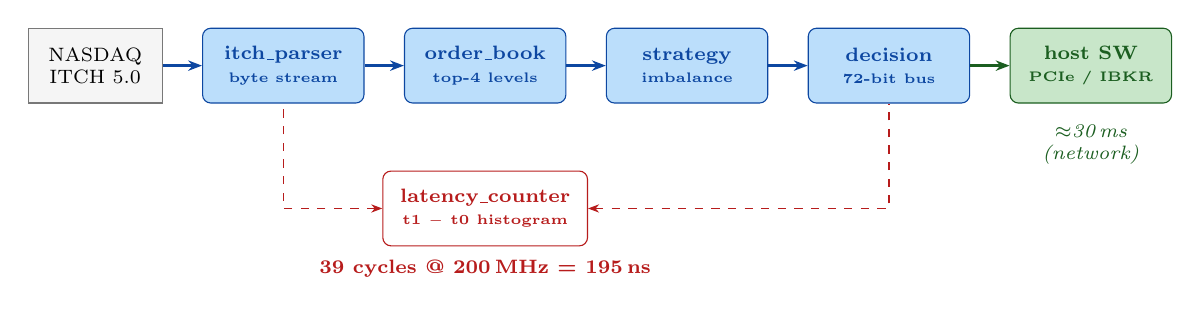
\begin{tikzpicture}[node distance=0.5cm and 0.5cm]
  \node[io]      (feed)   {NASDAQ\\ITCH 5.0};
  \node[blk, right=of feed] (parse) {itch\_parser\\{\tiny byte stream}};
  \node[blk, right=of parse] (book) {order\_book\\{\tiny top-4 levels}};
  \node[blk, right=of book] (strat) {strategy\\{\tiny imbalance}};
  \node[blk, right=of strat] (dec)  {decision\\{\tiny 72-bit bus}};
  \node[hostblk, right=of dec] (host) {host SW\\{\tiny PCIe / IBKR}};

  \draw[fa] (feed)  -- (parse);
  \draw[fa] (parse) -- (book);
  \draw[fa] (book)  -- (strat);
  \draw[fa] (strat) -- (dec);
  \draw[ga] (dec)   -- (host);

  \node[blk, fill=white, draw=accent, text=accent, below=0.85cm of book,
        minimum width=2.6cm] (lat) {latency\_counter\\{\tiny t1 $-$ t0 histogram}};
  \draw[{Stealth[length=4pt]}-, accent, dashed] (lat.west) -| (parse.south);
  \draw[{Stealth[length=4pt]}-, accent, dashed] (lat.east) -| (dec.south);

  \node[font=\scriptsize\itshape, hostgreen, below=0.15cm of host, align=center]
        {$\approx$30\,ms\\(network)};
  \node[font=\scriptsize\bfseries, accent, below=0.05cm of lat]
        {39 cycles @ 200\,MHz = 195\,ns};
\end{tikzpicture}
\end{center}

\vspace{-4pt}
\begin{itemize}[leftmargin=1.2em, itemsep=1pt, topsep=1pt]
  \item \textbf{One clock domain, one direction.} A byte enters every cycle; a decision
        leaves a fixed 39 cycles after a message completes. No floating-point anywhere in
        the data path --- all fixed-point integer arithmetic.
  \item \textbf{Valid/ready back-pressure} between the parser and the book means a message
        arriving while the book is busy is \emph{held}, never dropped.
  \item \textbf{An on-chip cycle counter} stamps the entry and exit of every message, so
        latency is \emph{measured}, not estimated --- and read back over AXI-Lite.
\end{itemize}

% ============================ PIPELINE STAGES ===============================
\section{Pipeline stages}

\begin{center}
\renewcommand{\arraystretch}{1.25}
\begin{tabular}{@{}>{\bfseries\raggedright\arraybackslash}p{3.45cm} p{7.7cm} >{\raggedleft\arraybackslash}p{2.6cm}@{}}
\toprule
\normalfont\bfseries Module & \normalfont\bfseries Role & \normalfont\bfseries Key property \\
\midrule
itch\_parser        & AXI-Stream byte decoder: turns a framed ITCH message into structured fields (type, timestamp, refs, side, shares, price). & 1 byte/cycle, held output \\
order\_book\_m2     & Direct-mapped 256-entry book; maintains the top 4 price levels per side, aggregating size at each level. & O(1) Add, RESCAN on edits \\
strategy\_imbalance & Depth-weighted book-imbalance signal with spread guard, cooldown and imbalance-scaled lot sizing. & 1 cycle, no division \\
latency\_counter    & Free-running cycle counter + 64-bucket histogram of tick-to-trade latency, read over AXI-Lite. & single-cycle precision \\
tick\_to\_trade\_top & Top-level wrapper: wires the four stages and packs the decision into a 72-bit bus. & 72-bit decision out \\
\bottomrule
\end{tabular}
\end{center}

\textbf{Decision bus (72 bits):} \texttt{[71:65]} reserved \textbullet\ \texttt{[64]} action
(0=BUY,\,1=SELL) \textbullet\ \texttt{[63:32]} limit price (fixed-point $\times$10{,}000)
\textbullet\ \texttt{[31:0]} size (shares). Read by the host over PCIe DMA, decoded, and
risk-checked before it reaches the broker.

% ============================ DESIGN DECISIONS ==============================
\section{Key design decisions}

\subsection{1. Determinism over throughput tricks}
The order book keeps top-of-book correct in \textbf{O(1)} on every Add. It only pays for a
full re-scan when an order \emph{at a displayed price level} is cancelled, deleted or
executed --- a cancel deep in the book is skipped entirely. Combined with the back-pressure
handshake, the result is a pipeline whose latency is a \textbf{single fixed number}, not a
distribution. A CPU, with its caches, interrupts and OS scheduler, cannot offer this; an
execution desk prices determinism directly.

\subsection{2. Fixed-point cross-multiply --- no dividers, no floats}
The imbalance test $\text{bid}/(\text{bid}{+}\text{ask})$ is never computed as a division.
It is rearranged into a cross-multiply, e.g. BUY when
$\text{bid\_size}\times 10 > \text{BID\_THRESH}\times\text{ask\_size}$. One DSP multiply per
side, one clock cycle, exact integer arithmetic --- no FPU, no multi-cycle divider, no
rounding error.

\subsection{3. The order book is RAM, not flip-flops}
The 256-entry $\times$ 130-bit order table is a memory, not 33{,}280 registers. The
per-slot ``occupied'' flag was pulled into a small separate bit-vector so the payload
infers distributed RAM with combinational (zero-cycle) reads --- keeping the book O(1)
\emph{and} synthesizable without exploding the flip-flop count.

\subsection{4. Correct capture at the message boundary (the NBA fix)}
When a field's last byte coincides with AXI-Stream \texttt{tlast}, a naive non-blocking
assignment captures the \emph{pre-shift} value and drops that byte. The parser computes
combinational ``next'' values that include the current byte, so the output latched at
\texttt{tlast} is always complete. This single subtlety was the root cause of the first
generation of failing tests.

% ============================ ITCH SUPPORT ==================================
\section{Market-data coverage}

Eight ITCH 5.0 message types are decoded. Replace carries \emph{two} order references and
shifted field offsets; Trade is informational (the book treats it as a no-op); Add-with-MPID
and Execute-with-Price reuse Add/Execute field positions.

\begin{center}
\renewcommand{\arraystretch}{1.12}
\begin{tabular}{@{}c l c l@{}}
\toprule
\textbf{Type} & \textbf{Message} & \textbf{Bytes} & \textbf{Effect on book} \\
\midrule
A & Add Order                 & 36 & insert order, update level \\
F & Add Order with MPID       & 40 & insert (same as A; MPID ignored) \\
X & Order Cancel              & 23 & reduce shares \\
D & Order Delete              & 19 & remove order \\
E & Order Executed            & 31 & reduce shares \\
C & Order Executed with Price & 36 & reduce shares (exec price logged) \\
U & Order Replace             & 35 & remove original, insert replacement \\
P & Trade (non-cross)         & 44 & none (informational print) \\
\bottomrule
\end{tabular}
\end{center}

% ============================ STRATEGY ======================================
\section{Strategy and risk controls}

The signal is short-horizon \textbf{book imbalance}, a well-known micro-structure predictor:
a bid much heavier than the ask anticipates an up-move (BUY), and vice-versa. Three controls
turn the raw signal into something an actual desk would run:

\begin{itemize}[leftmargin=1.2em, itemsep=1pt, topsep=1pt]
  \item \textbf{Depth-weighted volume.} Imbalance is computed over the top 4 levels, weighting
        the touch most heavily (weight 4) down to the deepest tracked level (weight 1) --- so a
        \emph{supported} bid fires even when the touch alone looks balanced.
  \item \textbf{Spread guard.} No trade unless the book is well-formed (ask\,$>$\,bid) and the
        spread is within \texttt{MAX\_SPREAD\_TICKS} ($\$0.10$) --- avoids chasing fills in thin
        or locked markets.
  \item \textbf{Cooldown + scaled sizing.} After firing, new decisions are suppressed for
        \texttt{COOLDOWN\_CYCLES} (no order spam); order size scales with imbalance strength
        from \texttt{BASE\_LOT}=100 up to \texttt{MAX\_LOT}=250 shares.
\end{itemize}

Off-chip, \texttt{risk\_guard.py} applies pre-trade checks (SEC Rule 15c3-5) before any
order is sent, and the live path only ever targets a paper account.

% ============================ LATENCY MEASUREMENT ===========================
\section{Latency measurement (how the 195\,ns is proven)}

A free-running 32-bit counter timestamps \texttt{t0} on the first byte of a message and
\texttt{t1} on \texttt{decision\_valid}; $\Delta = t1-t0$ is binned into a 64-bucket
histogram. Because the pipeline is deterministic, that histogram is a \textbf{single spike}
at 39 cycles --- visual proof of zero jitter, where a CPU would smear across 3--4 orders of
magnitude. The host reads it over a small AXI-Lite slave:

\begin{center}
\renewcommand{\arraystretch}{1.1}
\begin{tabular}{@{}l l l@{}}
\toprule
\textbf{Address} & \textbf{Register} & \textbf{Access} \\
\midrule
\texttt{0x000 -- 0x0FC} & histogram buckets 0--63 & read \\
\texttt{0x100}          & last measured latency (cycles) & read \\
\texttt{0x104}          & clear (write 1 to reset) & write \\
\bottomrule
\end{tabular}
\end{center}

% ============================ VERIFICATION ==================================
\section{Verification}

Every RTL output is diffed \textbf{bit-for-bit} against an independent Python golden model
(\texttt{golden/itch\_parser.py}) under cocotb + QuestaSim. The same generated vectors drive
both implementations; any field mismatch fails the test. All RTL also passes a strict
\texttt{verilator -Wall} lint.

\begin{center}
\renewcommand{\arraystretch}{1.12}
\begin{tabular}{@{}l c l@{}}
\toprule
\textbf{Testbench} & \textbf{Tests} & \textbf{Covers} \\
\midrule
tb\_itch\_parser        & 11 & all 8 message types, back-to-back, back-pressure hold \\
tb\_order\_book         & 11 & M1 top-of-book on Add (baseline) \\
tb\_order\_book\_m2     & 28 & multi-level depth, RESCAN, replace, RESCAN-skip, no-op trade \\
tb\_strategy\_imbalance & 21 & imbalance, spread guard, cooldown, lot tiers, depth weighting \\
tb\_latency\_counter    &  5 & histogram, saturation, AXI-Lite read, clear \\
tb\_tick\_to\_trade     &  5 & full pipeline, 195\,ns latency, back-pressure no-drop \\
\midrule
\textbf{Total}          & \textbf{81} & \textbf{100\,\% pass} \\
\bottomrule
\end{tabular}
\end{center}

% ============================ HARD NUMBERS ==================================
\section{Hard numbers}

\begin{center}
\renewcommand{\arraystretch}{1.2}
\begin{tabular}{@{}>{\raggedright\arraybackslash}p{6.0cm} >{\raggedright\arraybackslash}p{4.2cm} r@{}}
\toprule
\textbf{Metric} & \textbf{This design (FPGA)} & \textbf{Software path} \\
\midrule
Tick-to-trade latency        & \textbf{195\,ns} (39 cycles)      & $\sim$30{,}000{,}000\,ns (30\,ms) \\
Latency jitter               & \textbf{0\,ns} (deterministic)    & milliseconds, unbounded \\
Speed-up to a decision       & \multicolumn{2}{l}{\textbf{$>$150{,}000$\times$} faster} \\
Clock frequency              & 200\,MHz (5\,ns period)           & --- \\
ITCH ingest rate             & 1 byte/cycle = \textbf{200\,MB/s} & --- \\
Order book                   & top-4 levels/side, 256 live orders & --- \\
ITCH message types decoded   & 8 (A, F, C, D, E, U, X, P)         & --- \\
Data-path arithmetic         & fixed-point, \textbf{0 floats}     & --- \\
Verification                 & \textbf{81/81} tests, golden-model diff & --- \\
\bottomrule
\end{tabular}
\end{center}

% ============================ STATUS ========================================
\section{Status and honest claims}

\begin{center}
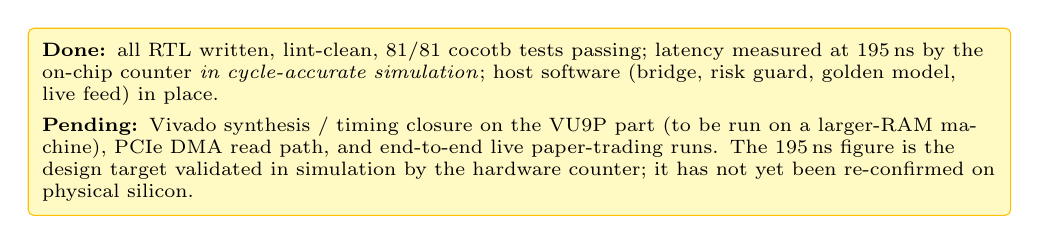
\begin{tikzpicture}
\node[note, text width=\linewidth]{%
\textbf{Done:} all RTL written, lint-clean, 81/81 cocotb tests passing; latency
measured at 195\,ns by the on-chip counter \emph{in cycle-accurate simulation}; host
software (bridge, risk guard, golden model, live feed) in place.\\[3pt]
\textbf{Pending:} Vivado synthesis / timing closure on the VU9P part (to be run on a
larger-RAM machine), PCIe DMA read path, and end-to-end live paper-trading runs. The
195\,ns figure is the design target validated in simulation by the hardware counter; it
has not yet been re-confirmed on physical silicon.%
};
\end{tikzpicture}
\end{center}

\vspace{2pt}
\textbf{Toolchain:} SystemVerilog RTL \textbullet\ cocotb 2.x + QuestaSim 2021.2 \textbullet\
Verilator lint \textbullet\ Vivado ML (synthesis) \textbullet\ Python golden model + IBKR
\texttt{ib\_async}. \quad \textbf{Target:} AWS F1 \texttt{f1.2xlarge}, Xilinx UltraScale+ VU9P.

\vfill
\hruleline
{\footnotesize\color{rulegray}
Detail documents: \textbf{Part 1} --- Foundation \& Architecture \textbullet\
\textbf{Part 2} --- RTL Design \& Verification \textbullet\
\textbf{Part 3} --- Integration \& Deployment.}

\end{document}
